



\documentclass[
	% -- opções da classe memoir --
	12pt,				% tamanho da fonte
	openright,			% capítulos começam em pág ímpar (insere página vazia caso preciso)
	oneside,			% para impressão em recto e verso. Oposto a oneside
	a4paper,			% tamanho do papel. 
	% -- opções da classe abntex2 --
	%chapter=TITLE,		% títulos de capítulos convertidos em letras maiúsculas
	%section=TITLE,		% títulos de seções convertidos em letras maiúsculas
	%subsection=TITLE,	% títulos de subseções convertidos em letras maiúsculas
	%subsubsection=TITLE,% títulos de subsubseções convertidos em letras maiúsculas
	% -- opções do pacote babel --
	english,			% idioma adicional para hifenização
	french,				% idioma adicional para hifenização
	spanish,			% idioma adicional para hifenização
	brazil				% o último idioma é o principal do documento
	]{abntex2}




% Pacotes básicos 
\usepackage{lmodern}			% Usa a fonte Latin Modern			
\usepackage[T1]{fontenc}		% Selecao de codigos de fonte.
\usepackage[utf8]{inputenc}		% Codificacao do documento (conversão automática dos acentos)
\usepackage{indentfirst}		% Indenta o primeiro parágrafo de cada seção.
\usepackage{color}				% Controle das cores
\usepackage{graphicx}			% Inclusão de gráficos
\usepackage{microtype} 			% para melhorias de justificação
\usepackage{amsmath}			% lib para equacoes
\usepackage{svg}
\usepackage{pythonhighlight}
%\usepackage{float}


% Pacotes adicionais, usados apenas no âmbito do Modelo Canônico do abnteX2

\usepackage{lipsum}				% para geração de dummy text



% Pacotes de citações
\usepackage[num, backend=biblatex]{abntex2cite}	% Citações padrão ABNT
\usepackage[brazilian,hyperpageref]{backref}	 % Paginas com as citações na bibl


 
% CONFIGURAÇÕES DE PACOTES

% Configurações do pacote backref
% Usado sem a opção hyperpageref de backref
\renewcommand{\backrefpagesname}{Citado na(s) página(s):~}
% Texto padrão antes do número das páginas
\renewcommand{\backref}{}
% Define os textos da citação
\renewcommand*{\backrefalt}[4]{
	\ifcase #1 %
		Nenhuma citação no texto.%
	\or
		Citado na página #2.%
	\else
		Citado #1 vezes nas páginas #2.%
	\fi}%
% ---



% ---
% Informações de dados para CAPA e FOLHA DE ROSTO
% ---
\titulo{Robô omnidirecional de 3 rodas}
\autor{Daniel Ermelino Carvalho \\ Lucas Pereira Lima}
\local{Brasil}
\data{2022}
\orientador{Marcelo Bender Perotoni}
\instituicao{%
  Universidade Federal do ABC
  \par
  CECS
  \par
   Engenharia de Instrumentação, Automação e Robótica}
\tipotrabalho{Tese (Doutorado)}
% O preambulo deve conter o tipo do trabalho, o objetivo, 
% o nome da instituição e a área de concentração 
\preambulo{ }



% Configurações de aparência do PDF final

% alterando o aspecto da cor azul
\definecolor{blue}{RGB}{5,5,180}

% informações do PDF
\makeatletter
\hypersetup{
     	%pagebackref=true,
		pdftitle={\@title}, 
		pdfauthor={\@author},
    	pdfsubject={\imprimirpreambulo},
	    pdfcreator={LaTeX with abnTeX2},
		pdfkeywords={abnt}{latex}{abntex}{abntex2}{trabalho acadêmico}, 
		colorlinks=true,       		% false: boxed links; true: colored links
    	linkcolor=blue,          	% color of internal links
    	citecolor=blue,        		% color of links to bibliography
    	filecolor=magenta,      		% color of file links
		urlcolor=blue,
		bookmarksdepth=4
}
\makeatother


% Posiciona figuras e tabelas no topo da página quando adicionadas sozinhas
% em um página em branco. Ver https://github.com/abntex/abntex2/issues/170
\makeatletter
\setlength{\@fptop}{5pt} % Set distance from top of page to first float
\makeatother



% Possibilita criação de Quadros e Lista de quadros.
% Ver https://github.com/abntex/abntex2/issues/176

\newcommand{\quadroname}{Quadro}
\newcommand{\listofquadrosname}{Lista de quadros}

\newfloat[chapter]{quadro}{loq}{\quadroname}
\newlistof{listofquadros}{loq}{\listofquadrosname}
\newlistentry{quadro}{loq}{0}

% configurações para atender às regras da ABNT
\setfloatadjustment{quadro}{\centering}
\counterwithout{quadro}{chapter}
\renewcommand{\cftquadroname}{\quadroname\space} 
\renewcommand*{\cftquadroaftersnum}{\hfill--\hfill}

\setfloatlocations{quadro}{hbtp} % Ver https://github.com/abntex/abntex2/issues/176


% Espaçamentos entre linhas e parágrafos 


% O tamanho do parágrafo é dado por:
\setlength{\parindent}{1.3cm}

% Controle do espaçamento entre um parágrafo e outro:
\setlength{\parskip}{0.2cm}  % tente também \onelineskip


% compila o indice
\makeindex




% Início do documento
\begin{document}

% Seleciona o idioma do documento (conforme pacotes do babel)
%\selectlanguage{english}
\selectlanguage{brazil}

% Retira espaço extra obsoleto entre as frases.
\frenchspacing 


% ELEMENTOS TEXTUAIS
\textual

	% Capitulo com exemplos de comandos inseridos de arquivo externo 
	\include{abntex2-modelo-include-comandos}

	\chapter{Projeto 1}
		Daniel Ermelino Carvalho - RA 11092613

		link de arquivos:
		\url{https://github.com/dcarve/data_visulization_ufabc/tree/main/praticas/pratica_2}
	
	\chapter{Preparação de Dados}

\subsection*{}
Embora seja possível usar o tableau para preparar os dados, como por exemplo fazer join com a tabela Orders e People, 
era mais vantajoso preparar o dado com python anteriormente, pois também seria necessário um tratamento dos dados de cotações para a questão N2,
tratamento que seria mais complicado de fazer no tableau.
Então optei por preprar os dados antes, e depois importa-los para o tableau.

\subsection*{Código do etl}

\begin{python}

import pandas as pd
import re
import numpy as np

superstore_orders = pd.read_excel(
    "VIS_Pr_02_Superstore.xls",
    sheet_name="Orders"
)
superstore_people = pd.read_excel(
    "VIS_Pr_02_Superstore.xls",
    sheet_name="People"
)
cotacao = pd.read_csv("VIS_Pr_02_euro_cotacao_99_22.csv")

cotacao = cotacao[[
    "Period\\Unit:",
    "[US dollar ]",
    "[Chinese yuan renminbi ]"
]]

cotacao.columns = ["period", "dollar", "yuan"]

pattern = re.compile(r"[+-]?([0-9]*[.])?[0-9]+")

cotacao["dollar"] = cotacao.apply(
    lambda row: 
        row["dollar"] 
        if pattern.match(str(row["dollar"]))
        else np.nan,
    axis=1
)
cotacao["yuan"] = cotacao.apply(
    lambda row: 
        row["yuan"]
        if pattern.match(str(row["yuan"]))
        else np.nan,
    axis=1
)

cotacao["euro"] = 1
cotacao["dollar"] = cotacao['dollar'].astype(float)
cotacao["yuan"] = cotacao['yuan'].astype(float)

cotacao["euro"] = cotacao["euro"]/cotacao["dollar"]
cotacao["yuan"] = cotacao["yuan"] * cotacao["euro"]
cotacao["dollar"] = 1

cotacao["period"] = pd.to_datetime(cotacao["period"])

cotacao = cotacao.groupby(
    cotacao["period"].dt.to_period("Q")
)[
    "dollar",
    "euro",
    "yuan"
].mean().reset_index()

superstore_orders["period"] = superstore_orders["Order Date"].dt.to_period("Q")

superstore_orders = superstore_orders.merge(
    cotacao,
    on="period",
    how="left"
)
superstore_orders = superstore_orders.merge(
    superstore_people,
    on="Region",
    how="left"
)

superstore_orders = superstore_orders[[
    "Order Date",
    "Country",
    "City",
    "State",
    "Postal Code",
    "Region",
    "Category",
    "Sub-Category",
    "Sales",
    "Quantity",
    "Discount",
    "Profit",
    "period",
    "dollar",
    "euro",
    "yuan",
    "Person"
]]

superstore_orders.to_csv("superstore_etl.csv")
\end{python}




	\chapter{N1}

\subsection*{Erros de servidor do tableau public}
O tableu public não estava permitindo publicar os dash, erro de servidor, então esse documento irá apresentar somente as imagens dos dashs.

\begin{figure}[h]
	\centering
	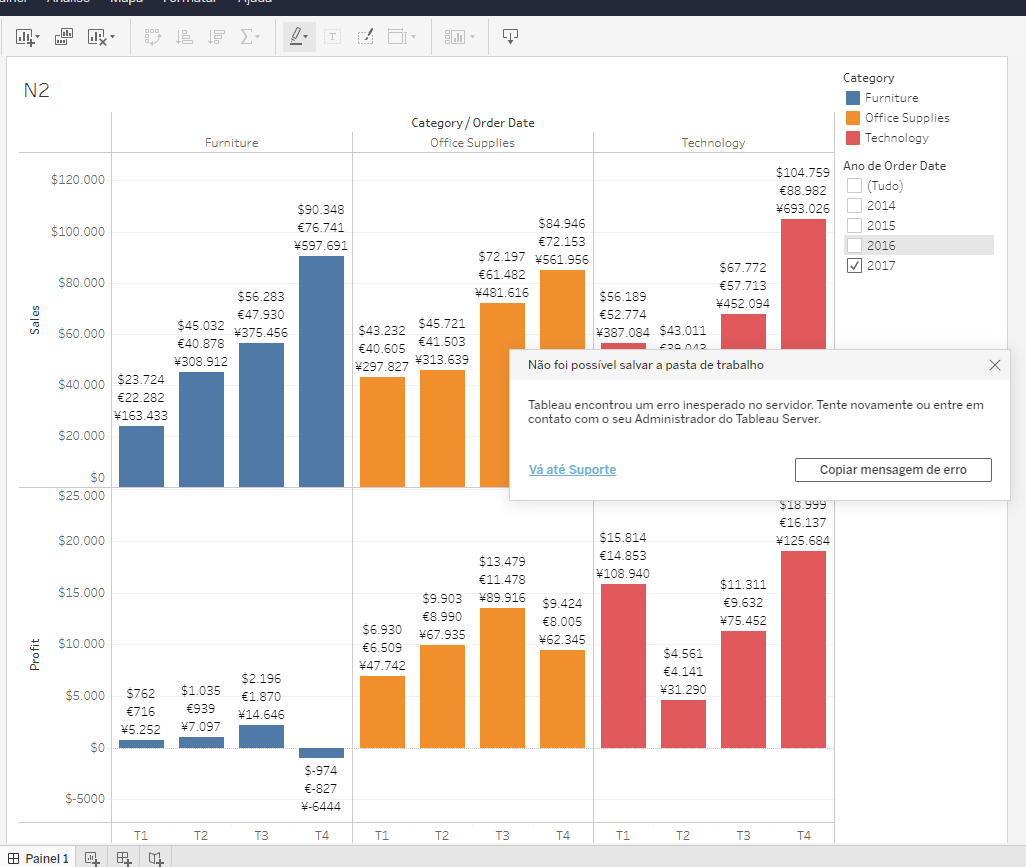
\includegraphics[width=\textwidth,keepaspectratio]{figures/erro_servidor_2}
	\caption{Erro no Tableau Public [2]}
	\label{lof}
\end{figure}


\subsection*{Dash da questão N1}
\begin{figure}[h]
	\centering
	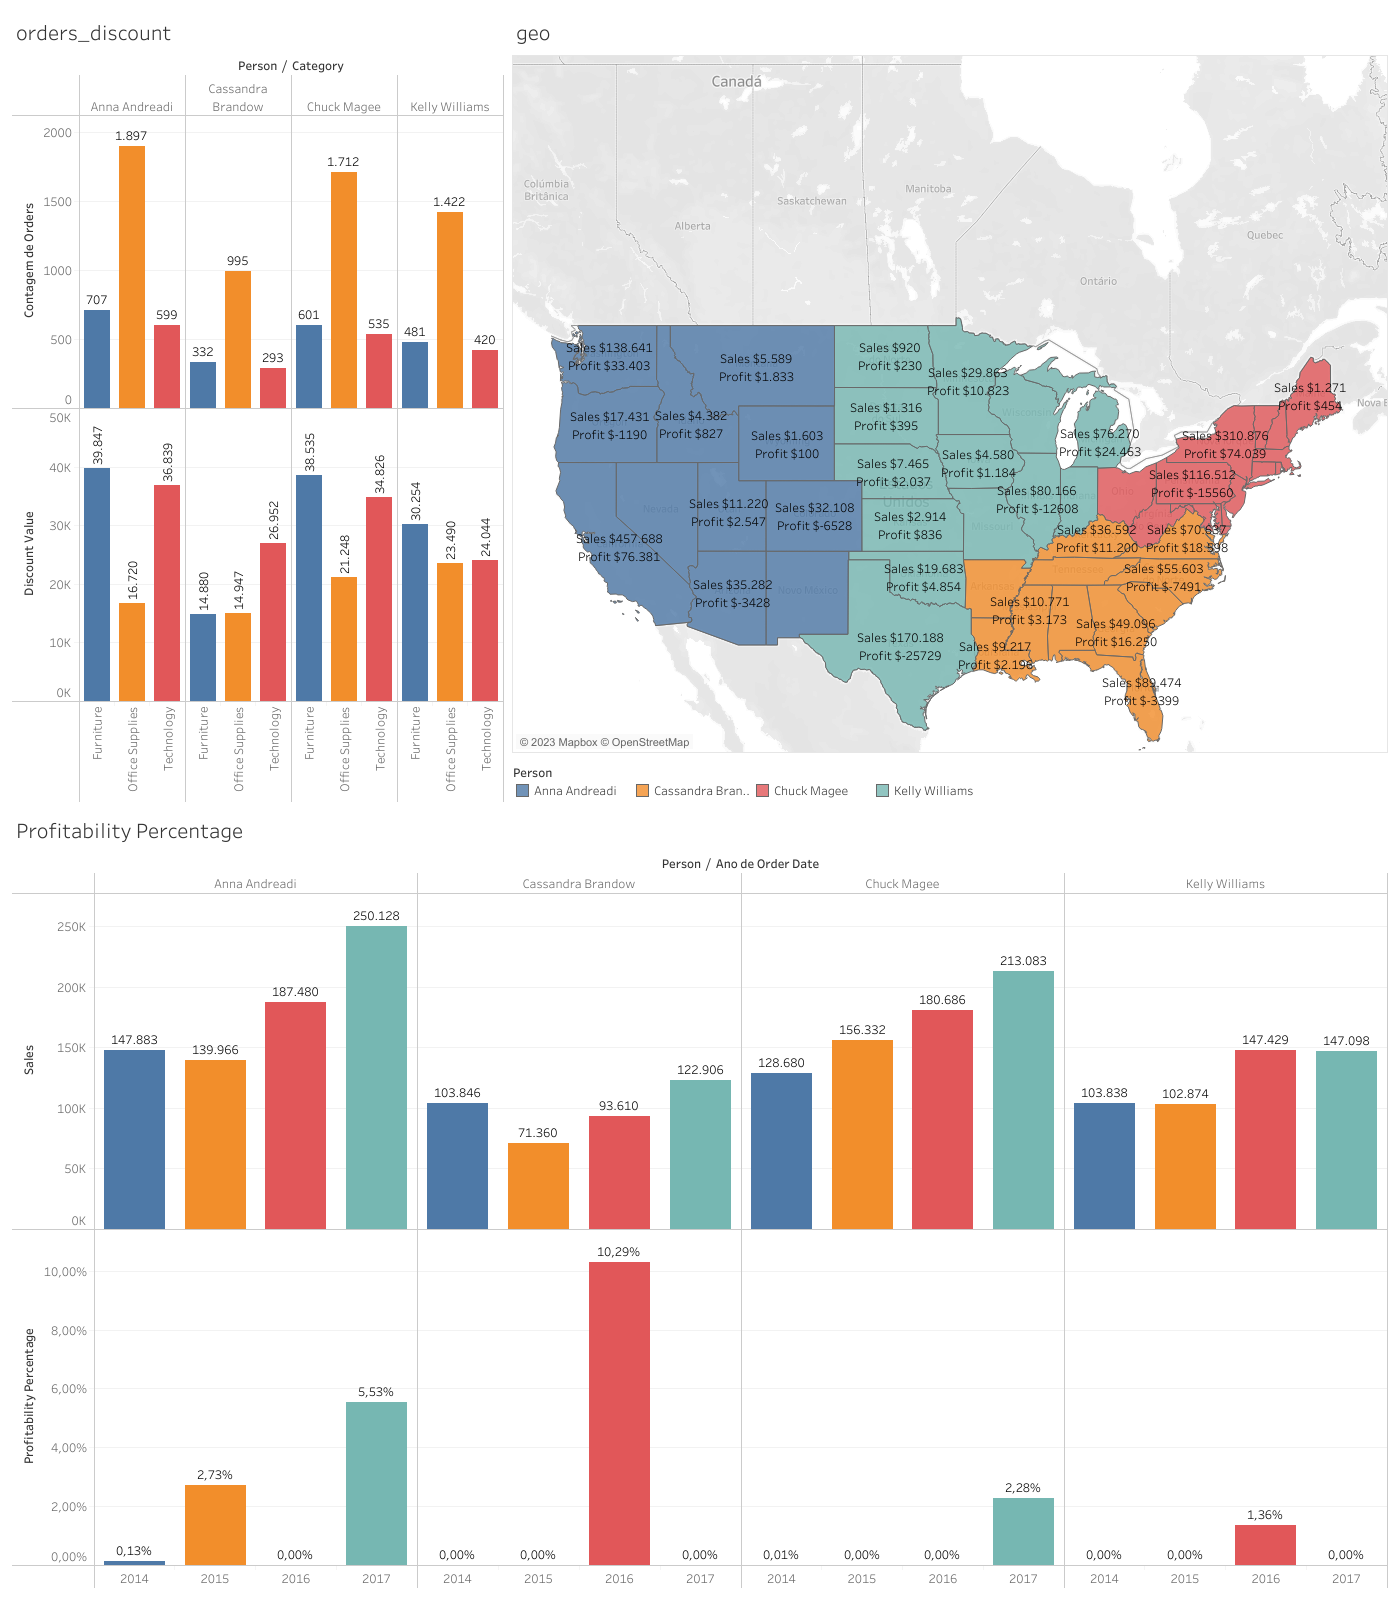
\includegraphics[width=\textwidth,keepaspectratio]{figures/n1_dash}
	\caption{Dash N1}
	\label{lof}
\end{figure}

	\chapter{N2}

\subsection*{Dash da questão N2}
\begin{figure}[h]
	\centering
	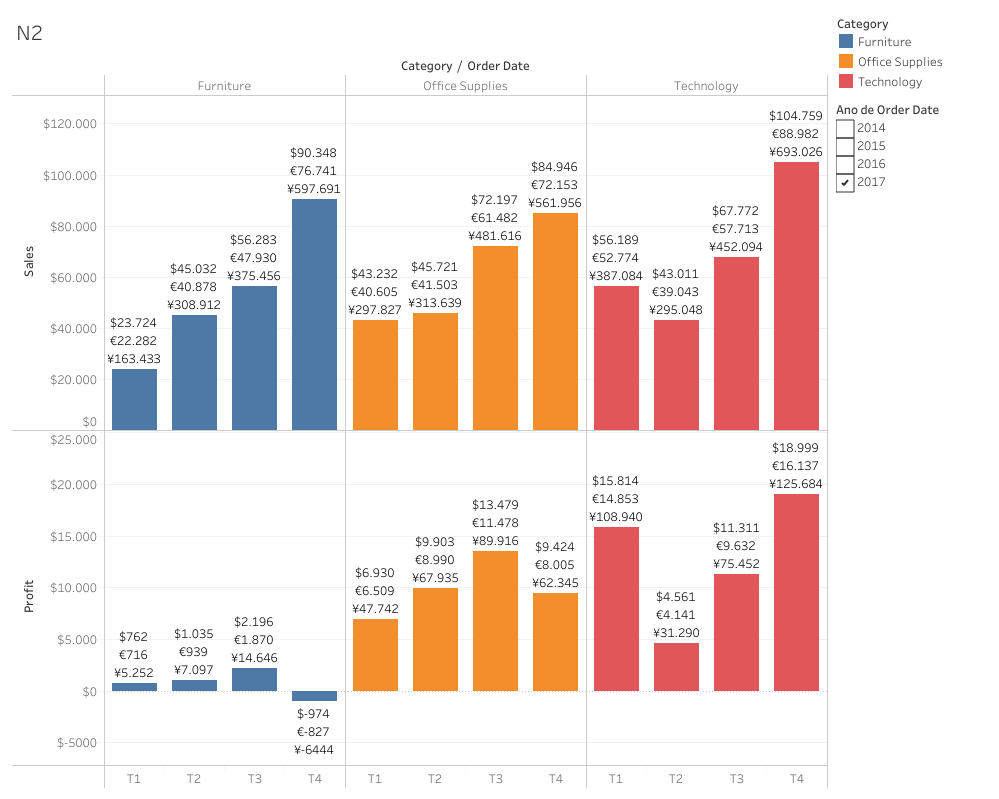
\includegraphics[width=\textwidth,keepaspectratio]{figures/n2_dash}
	\caption{Dash N2}
	\label{lof}
\end{figure}


	% ----------------------------------------------------------
	% Finaliza a parte no bookmark do PDF
	% para que se inicie o bookmark na raiz
	% e adiciona espaço de parte no Sumário
	% ----------------------------------------------------------
	\phantompart

%---------------------------------------------------------------------
% INDICE REMISSIVO
%---------------------------------------------------------------------
\phantompart
\printindex


\end{document}

